\documentclass[aspectratio=169,11pt]{beamer}

\usetheme{Madrid}
\usecolortheme{default}
\usefonttheme{professionalfonts}
\setbeamertemplate{navigation symbols}{}
\setbeamertemplate{footline}[frame number]

\usepackage{amsmath, amssymb, booktabs, graphicx}

\title{Labor Market Facts, Measurement, and Canonical Questions}
\subtitle{Labor I --- Week 1}
\author{Teaching deck draft}
\date{}

\begin{document}

\begin{frame}
  \titlepage
\end{frame}

\begin{frame}{Week 1 question}
\begin{itemize}
    \item Which measured labor-market objects organize the rest of Labor I and Labor II?
    \item How much interpretation is already fixed by the way those objects are constructed?
    \item Why are descriptive facts part of identification rather than just background?
\end{itemize}
\end{frame}

\begin{frame}{The field starts with a short list of objects}
\begin{itemize}
    \item Employment, unemployment, labor-force participation
    \item Hours, hourly wages, weekly earnings, compensation
    \item Worker transitions across states, jobs, and firms
    \item Group gaps and dispersion
\end{itemize}

\medskip
Four Week 1 distinctions: stocks versus flows, prices versus quantities, worker outcomes versus firm outcomes, levels versus composition-adjusted change.
\end{frame}

\begin{frame}{Measurement map}
\small
\begin{tabular}{p{0.22\linewidth} p{0.27\linewidth} p{0.39\linewidth}}
\toprule
Object & Unit & Why it matters \\
\midrule
Employment / unemployment / LFPR & Person-month & Extensive-margin attachment and slack \\
Hours worked & Worker-week or year & Intensive margin conditional on work \\
Hourly wage & Worker-job or worker-week & Price of labor \\
Weekly earnings & Worker-week & Wage plus hours \\
Compensation & Job or worker-job & Total reward, not just cash pay \\
Transitions & Matched month or linked records & Flows, mobility, frictions \\
\bottomrule
\end{tabular}
\end{frame}

\begin{frame}{Labor-market accounting identity}
\[
\frac{E_t}{P_t} = \frac{L_t}{P_t}\left(1-u_t\right)
\]

\begin{itemize}
    \item Employment-population ratio bundles participation and employment conditional on labor-force attachment.
    \item A decline in employment can come from weaker participation, weaker job finding, or both.
    \item Week 2 labor supply and later friction models reuse exactly this accounting.
\end{itemize}
\end{frame}

\begin{frame}{Labor-market status dashboard}
\begin{center}
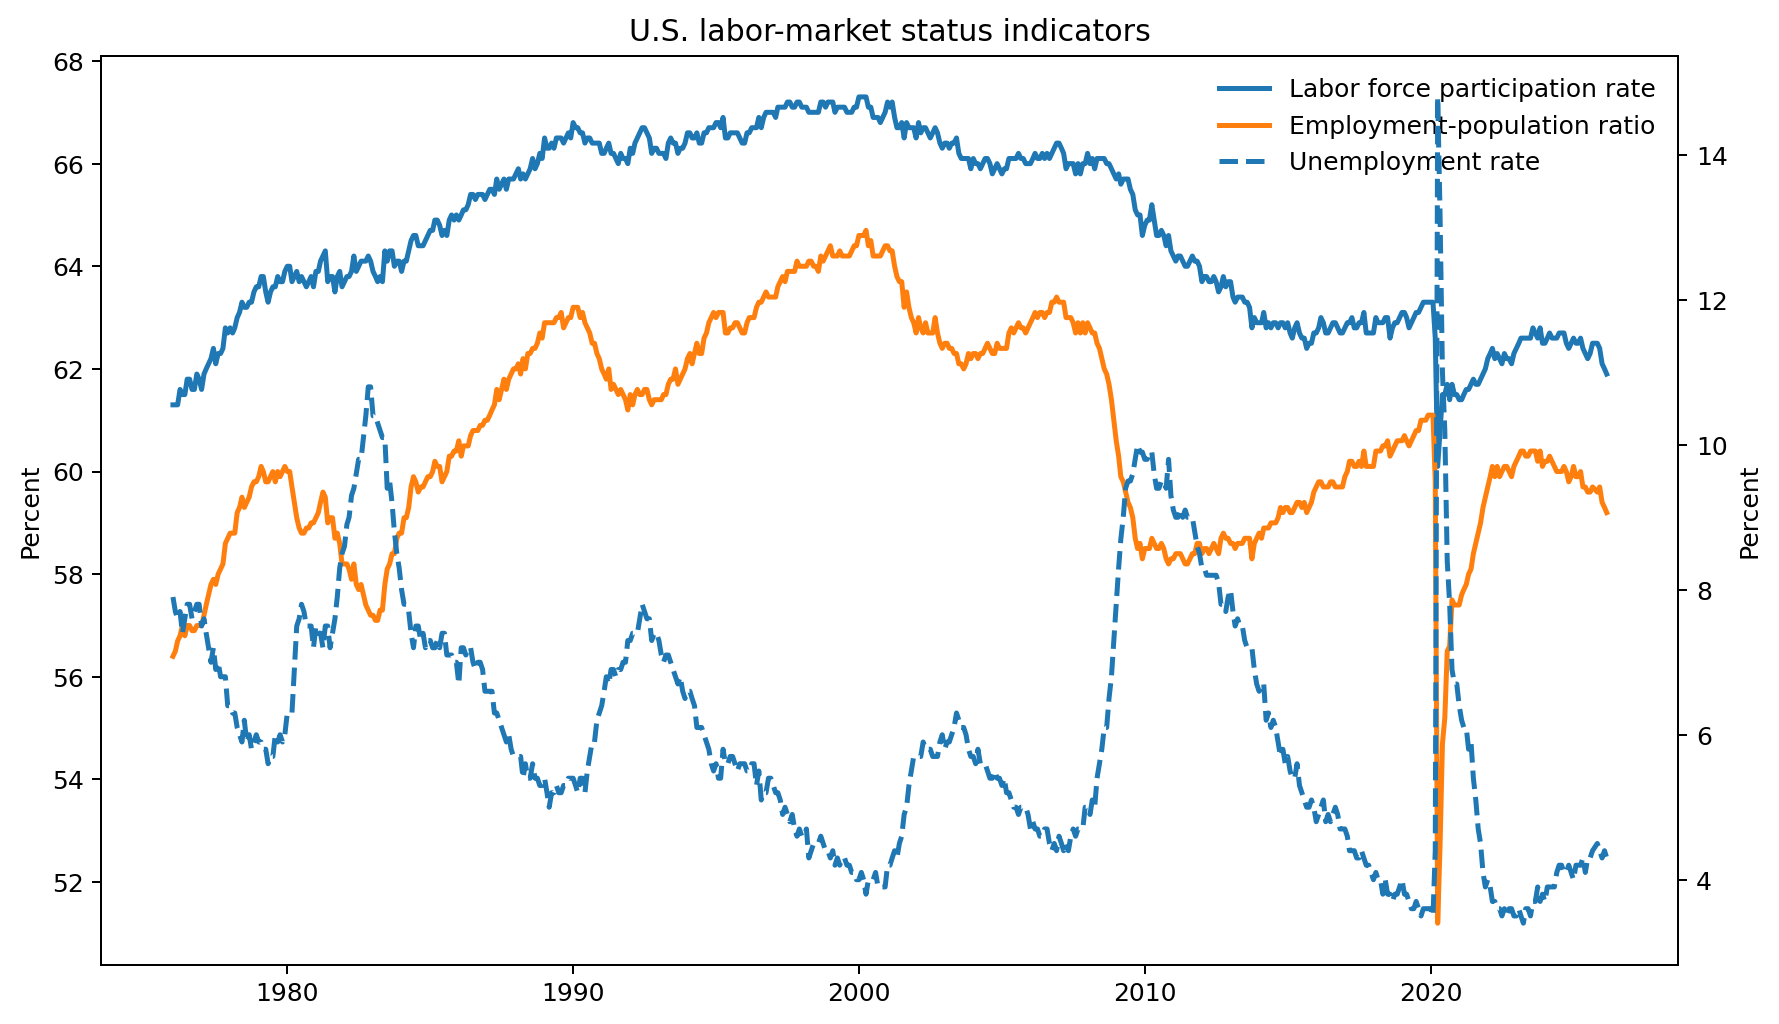
\includegraphics[width=0.9\linewidth]{../../assets/figures/01-labor-market-status-dashboard.png}
\end{center}
\end{frame}

\begin{frame}{Composition versus within-group wage change}
\[
\Delta \bar{w}_t
=
\sum_g \left(s_{gt} - s_{g,t-1}\right)\bar{w}_{g,t-1}
+
\sum_g s_{g,t-1}\left(\bar{w}_{gt} - \bar{w}_{g,t-1}\right)
+
R_t
\]

\begin{itemize}
    \item Aggregate wages move because worker shares change and because within-cell wages change.
    \item Week 1 should not call either object ``the wage'' without saying which one.
    \item This is the bridge to the Daly--Hobijn lab.
\end{itemize}
\end{frame}

\begin{frame}{Daly--Hobijn bridge}
\begin{center}
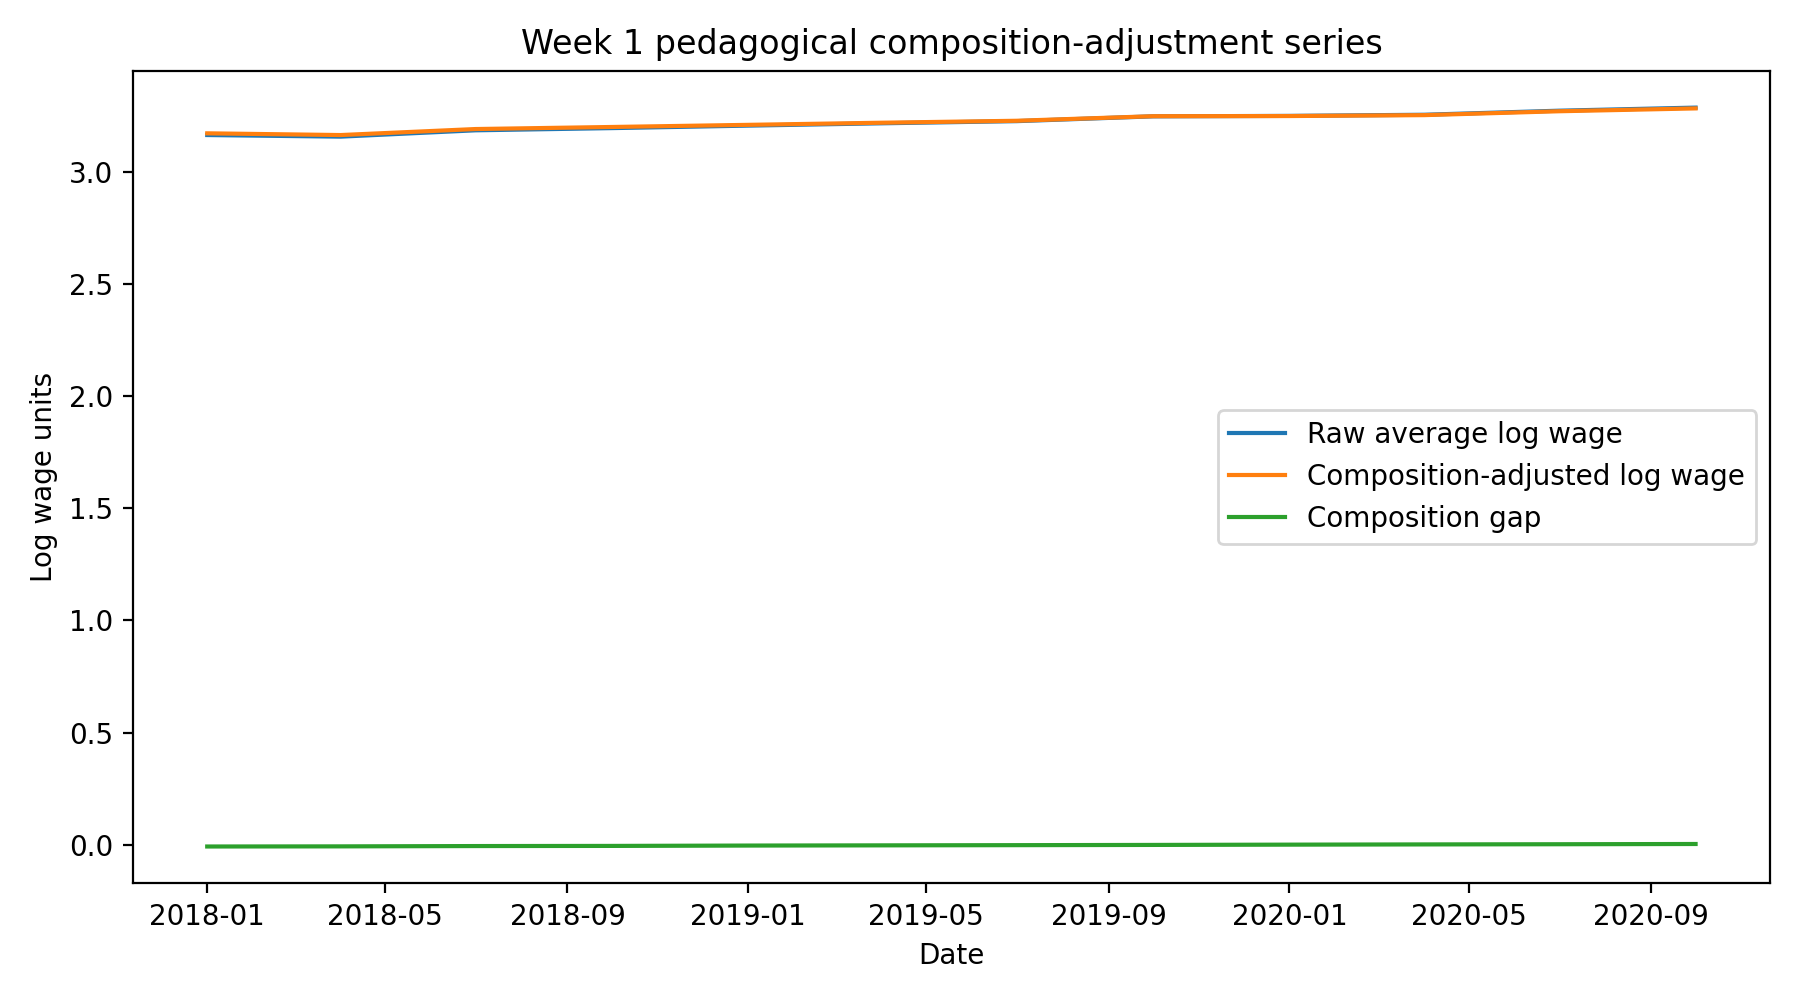
\includegraphics[width=0.84\linewidth]{../../labs/01-labor-market-facts/output/reproduced/composition_adjusted_series.png}
\end{center}
\end{frame}

\begin{frame}{What the opening facts do for the rest of the course}
\small
\begin{tabular}{p{0.32\linewidth} p{0.60\linewidth}}
\toprule
Week 1 object & Where it returns \\
\midrule
Employment-population ratio versus unemployment & Labor supply, aggregate adjustment, frictions \\
Weekly earnings versus hourly wages & Human capital, inequality, discrimination \\
Group heterogeneity in participation and pay & Households, gender, mobility, policy \\
Composition-adjusted versus raw wage growth & Business cycles, policy evaluation, code labs \\
Source choice and unit of observation & Methods and firm-side modules \\
\bottomrule
\end{tabular}
\end{frame}

\begin{frame}{Takeaways}
\begin{itemize}
    \item Week 1 is a map of recurring empirical objects, not a grab bag of facts.
    \item Measurement, description, mechanism, and identification should not be collapsed.
    \item Top-line aggregates are often mixtures of several margins.
    \item Later theories earn their place by explaining the objects defined here.
\end{itemize}
\end{frame}

\end{document}
